\documentclass[tikz,border=7pt]{standalone}
\usepackage{libertinus}
\usepackage{amsmath}
\usetikzlibrary{
  arrows.meta,
  backgrounds,
  calc,
  decorations.markings,
  fit,
  positioning
}

\definecolor{accent}{RGB}{38,103,115}
\definecolor{softgray}{RGB}{244,245,246}
\definecolor{midgray}{RGB}{123,128,132}

\tikzset{
  >={Latex[length=2.2mm,width=1.5mm]},
  flow/.style={-Latex,semithick,draw=black!72},
  accent flow/.style={-Latex,semithick,draw=accent},
  box/.style={
    draw=black!68,
    fill=softgray,
    rounded corners=1.2pt,
    align=center,
    inner xsep=5pt,
    inner ysep=4pt
  },
  accent box/.style={
    draw=accent,
    fill=accent!8,
    rounded corners=1.2pt,
    align=center,
    inner xsep=5pt,
    inner ysep=4pt
  },
  point/.style={circle,draw=black!75,fill=white,inner sep=1.7pt},
  accent point/.style={circle,draw=accent,fill=accent!10,inner sep=1.7pt},
  tinylabel/.style={font=\scriptsize,align=center},
  smalllabel/.style={font=\small,align=center},
  panel/.style={draw=black!28,rounded corners=2pt,inner sep=6pt}
}


\begin{document}
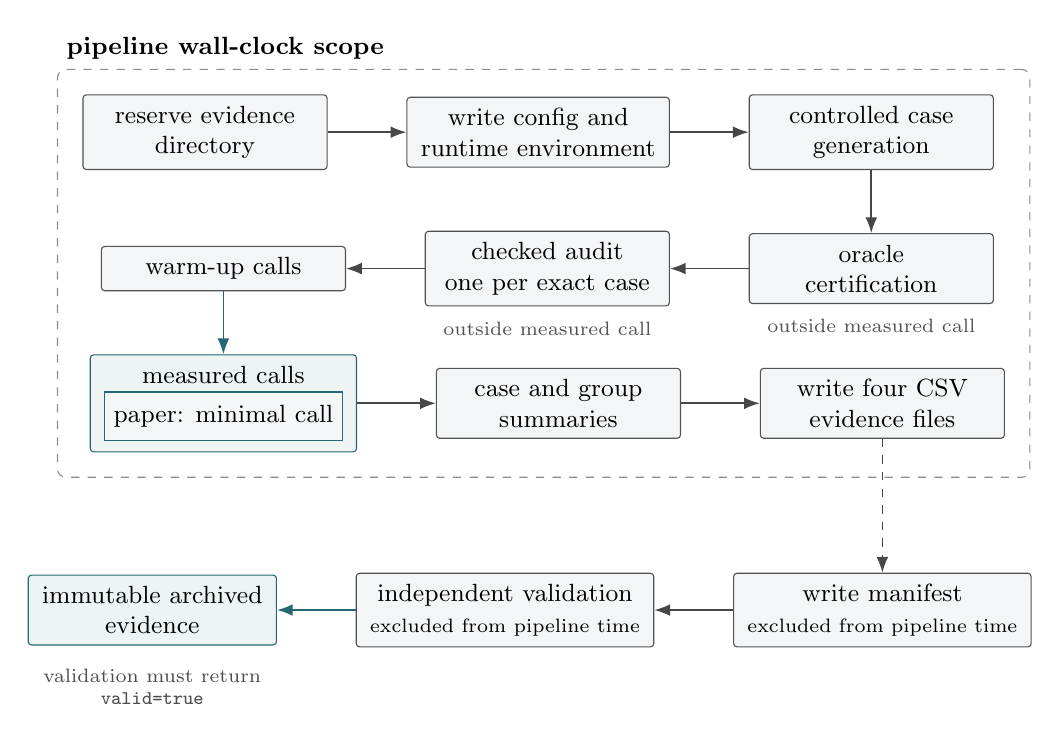
\begin{tikzpicture}[font=\small,node distance=8mm and 10mm]
  \node[box,minimum width=3.1cm] (reserve) {reserve evidence\\directory};
  \node[box,minimum width=3.1cm,right=of reserve] (config) {write config and\\runtime environment};
  \node[box,minimum width=3.1cm,right=of config] (generate) {controlled case\\generation};

  \node[box,minimum width=3.1cm,below=of generate] (oracle) {oracle\\certification};
  \node[box,minimum width=3.1cm,left=of oracle] (audit) {checked audit\\one per exact case};
  \node[box,minimum width=3.1cm,left=of audit] (warmup) {warm-up calls};

  \node[accent box,minimum width=3.1cm,below=of warmup] (measured) {
    measured calls\\[2pt]
    \fcolorbox{accent}{accent!5}{\strut paper: minimal call}
  };
  \node[box,minimum width=3.1cm,right=of measured] (summary) {case and group\\summaries};
  \node[box,minimum width=3.1cm,right=of summary] (csv) {write four CSV\\evidence files};

  \draw[flow] (reserve) -- (config);
  \draw[flow] (config) -- (generate);
  \draw[flow] (generate) -- (oracle);
  \draw[flow] (oracle) -- (audit);
  \draw[flow] (audit) -- (warmup);
  \draw[accent flow] (warmup) -- (measured);
  \draw[flow] (measured) -- (summary);
  \draw[flow] (summary) -- (csv);

  \node[tinylabel,text=black!68,below=2pt of oracle]
    {outside measured call};
  \node[tinylabel,text=black!68,below=2pt of audit]
    {outside measured call};

  \begin{scope}[on background layer]
    \node[draw=black!45,dashed,rounded corners=3pt,fit=(reserve)(generate)(oracle)(warmup)(measured)(csv),
      inner sep=9pt,label={[font=\small\bfseries,anchor=south west]north west:pipeline wall-clock scope}] (pipeline) {};
  \end{scope}

  \node[box,minimum width=3.1cm,below=17mm of csv] (manifest) {write manifest\\\scriptsize excluded from pipeline time};
  \node[box,minimum width=3.1cm,left=of manifest] (validate) {independent validation\\\scriptsize excluded from pipeline time};
  \node[accent box,minimum width=3.1cm,left=of validate] (archive) {immutable archived\\evidence};
  \draw[flow,dashed] (csv) -- (manifest);
  \draw[flow] (manifest) -- (validate);
  \draw[accent flow] (validate) -- (archive);

  \node[font=\scriptsize,align=center,text=black!70,below=5pt of archive]
    {validation must return\\\texttt{valid=true}};
\end{tikzpicture}
\end{document}
